\documentclass[12pt]{article}
\usepackage{amsmath}
\usepackage{graphicx}
\usepackage{color}
\title{Optimization Problem}
\begin{document}
\maketitle
\section{Problem Statement}
Our problem is to optimize metric, $M$, in the following scenario, we look at a few choices for $M$ below. Consider a data-center network abstracted as a complete bipartite graph with left vertices denoted by the set $A$ and right vertices denoted by $B$, each having $n$ elements. Flows arrive based on a schedule $S$ where flows are characterized by start time, size $(s_f)$, and $(a_i, b_i), i \in {1 \dots n}$, as the source and destination nodes, determine the schedule for flow processing that minimizes the metric $M$.
  
Examples of metric $M$ can be:
\begin{enumerate}
    \item Average flow completion time (FCT)
    \item Average slowdown (Normalize the FCT by the time it would take if it was the only flow in the network)
\end{enumerate}

\section{Tradeoff between algorithms}
\subsection{SRPT* - Extension of SRPT to our case}
SRPT scheduling is provably optimal for minimizing completion times on a single server. 
A natural extension of SRPT to this scenario is as follows. Consider a flow of size $size_f$ that arrives at $a$ destined to $b$. 
  \begin{description}
    \item[if] both ports are idle; schedule $f$
    \item[else if] only one of them is busy but $s_f$ is smaller than the flow on the busy port, schedule $f$ by pre-empting the other flow and check if any other flow can now be scheduled.
    \item[else if] both ports are busy and size($f$) is smaller, then schedule $f$ and pre-empt the other two flows; see if more flows can be scheduled.
  \end{description}

\subsection{Maximal Matching (MAXMAT)}
A maximal matching results in highest utilization possible. 


\begin{figure}[ht!]
   \centering
   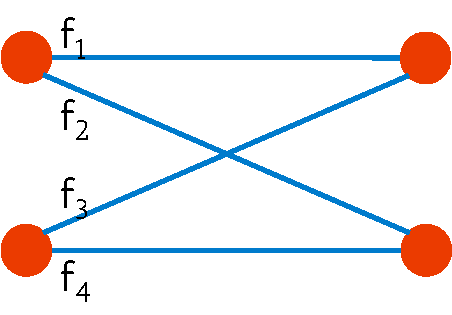
\includegraphics[width=3in]{Figures/SrptVsMaxMat.pdf}
   \caption{A simple example}
   \label{fig:fig1}
 \end{figure}

\subsection{SRPT* vs MAXMAT}
One can easily construct examples in which one is better than the other. Consider Figure \ref{fig:fig1} for a simple example. Assume at full line rate; a unit flow takes $1$ unit of time to finish. 



\subsubsection{SRPT* is better}
$t = 0$: $f_1$, $f_2$, $f_4$ come. $s_{f_1} = s_{f_4} = 10$, $s_{f_2} = 1$\\
If SRPT* is used, $f_2$ gets scheduled first and then $f_1$ and $f_4$: \\
\textbf{FCTs}: $f_1 = 11$, $f_2 = 1$, $f_4 = 11$; \textcolor{red}{Average = $23/3$}\\
\\
If MAXMAT is used: $f_1$ and $f_4$ get scheduled first and then $f_2$: \\
\textbf{FCTs}: $f_1 = 10$, $f_4 = 10$, $f_2 = 11$; \textcolor{red}{Average = $31/3$} 

\subsubsection{MAXMAT is better}
  $t = 0$: $f_1$, $f_4$ come. $s_{f_1} = s_{f_4} = 2 + e$   ($e$ is very small) \\
  $t = 1$: $f_2$ comes in with $s_{f_2} = 1$  \\
  $t = 2$: $f_3$ comes in with $s_{f_3} = 1$  \\
If SRPT* is used, $f_2$ preempts $f_1$ and $f_4$, then $f_3$ finishes and then $f_1$ and $f_4$ \\
\textbf{FCTs}: $f_1 = f_4 = 4+e$, $f_2 = 1$, $f_3 = 1$; \textcolor{red}{Average = $(10+e)/3$}\\
If MAXMAT is used used: $f_2$ and $f_3$ don’t preempt $f_1$ and $f_4$ \\
\textbf{FCTs}: $f_1 = f_4 = 2+e$, $f_2 = 2+e$, $f_3 = 1+e$; \textcolor{red}{Average = $(7+e)/3$}


\section{Optimality of Weighted Maximal Matching}
We consider the algorithm which schedules flows as per the weighted maximal matching where the weight of a flow, $w(f) = \frac{1}{s_f}$, i.e., reciprocal of flow's size. The weight of a matching is denoted by the sum of weight of the flows.

\begin{figure}[ht!]
   \centering
   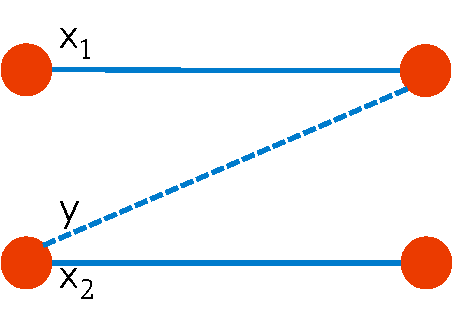
\includegraphics[width=3in]{Figures/wmaxmat.pdf}
   \caption{Optimality property of weighted maximal matching}
   \label{fig:fig2}
 \end{figure}


We are able to prove the following optimality in a local setting. Consider the scenario in Figure~\ref{fig:fig2}. Let $x_1 < x_2$ without loss of generality. We consider the following two schedules:
\begin{itemize}
	\item {\bf $A$}: Schedule $x_1$ and $x_2$ first. When $x_1$ finishes, check if $y$ would now pre-empt $x_2$. 
	\item {\bf $B$}: Schedule $y$ first and then $x_1$ and $x_2$
\end{itemize}

The sum of FCTs in $A$ is $x_1 + (y + x_2) + (x_1 + y)$ if $y$ pre-empts $x_2$ once $x_1$ finishes, which happens if $x_2 - x_1 > y$; otherwise it is $x_1 + x_2 + (x_2 + y)$.

The sum of FCTs in $B$ is $y + (y + x_1) + (y + x_2)$.

We show the following:
If $A \succ B$ then $w(A) > w(B)$. (The reverse side is straight forward which actually establishes equivalence).

Case 1: $x_2 - x_1 > y$:
$A \succ B \equiv x_1 < y$. Then $w(A) = \frac{1}{x_1} + \frac{1}{x_2} > \frac{1}{x_1} > \frac{1}{y} = w(B)$

Case 2: $x_2 - x_1 < y$:
$A \succ B \equiv x_2 < 2y$. Then $w(A) = \frac{1}{x_1} + \frac{1}{x_2} > 2\frac{1}{x_2} > 2\frac{1}{2y} = w(B)$

H.P.

\end{document}